\subsubsection{Set operationer}

Er operationer vi kan lave på tværs af forskellige Set, semantik er beskrevet ved hjælp af figur~\ref{fig:union_intersection_difference}. Eksempler på brug af disse kan ses på figur~\ref{fig:union_intersection_difference_example}.

\paragraph{Krav}

For at kunne udføre disse operationer skal nogle betingelser være opfyldt: 

\begin{itemize}
	\item Relationerne (tabellerne) skal have samme antal kolonner.
	\item Domænerne skal være ens (kolonnerne skal indeholde de samme type data).
\end{itemize}

\begin{figure}[H]
	\centering
	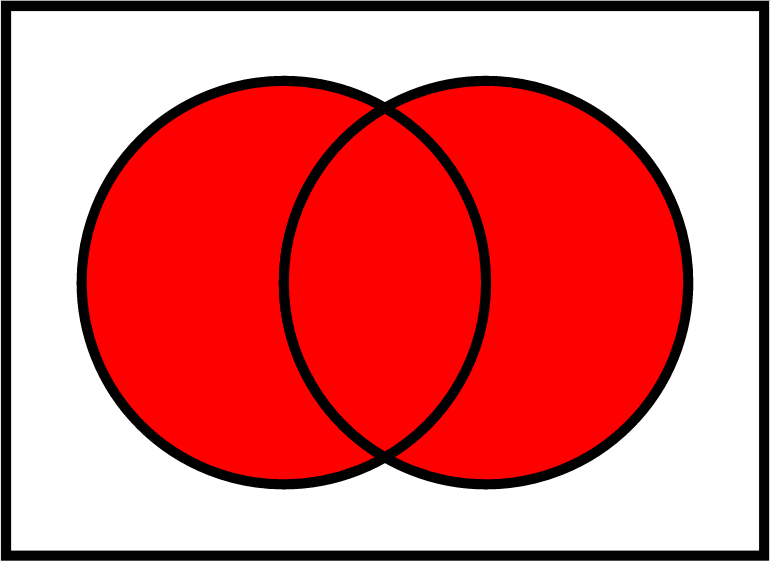
\includegraphics[width=.3\textwidth]{figs/spm6/union}\hfill
	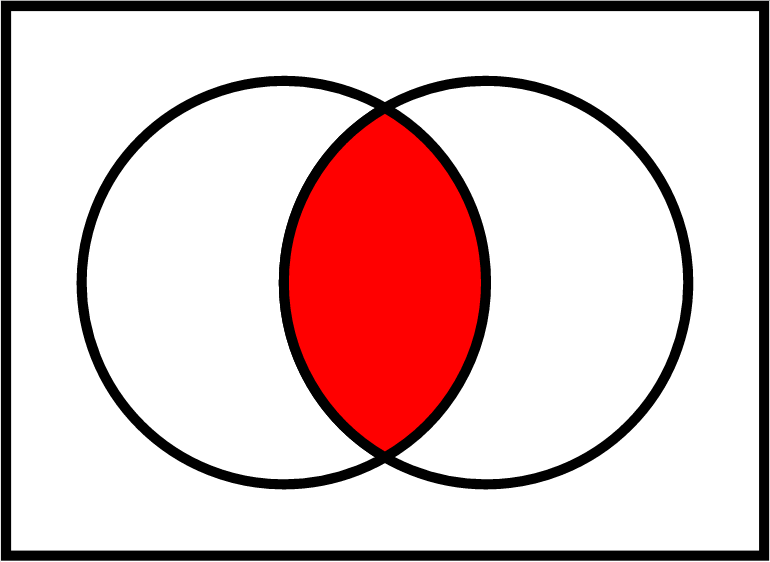
\includegraphics[width=.3\textwidth]{figs/spm6/intersection}\hfill
	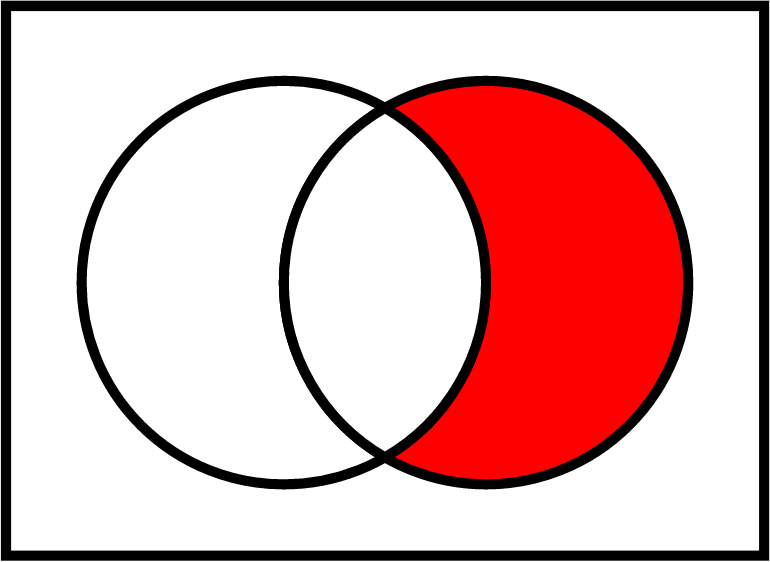
\includegraphics[width=.3\textwidth]{figs/spm6/difference}
	
	\caption{\href{https://en.wikipedia.org/wiki/Union_(set_theory)}{UNION} (tv), \href{https://en.wikipedia.org/wiki/Intersection_(set_theory)}{INTERSECTION} (midt) og \href{https://en.wikipedia.org/wiki/Complement_(set_theory)}{DIFFERNENCE} (tv).}
	\label{fig:union_intersection_difference}	
\end{figure}

Hvis vi har to relationer R og S (taget fra \href{http://db.grussell.org/section010.html#_Toc67114476}{udleveret materiale}). 

%\begin{itemize}
%	
%	\item \textbf{UNION of R and S:}\\
%	The union of two relations is a relation that includes all the tuples that are either in R or in S or in both R and S. Duplicate tuples are eliminated.
%	
%	\item \textbf{INTERSECTION of R and S:}\\
%	The intersection of R and S is a relation that includes all tuples that are both in R and S.
%	
%	\item \textbf{DIFFERENCE of R and S:}\\
%	The difference of R and S is the relation that contains all the tuples that are in R but that are not in S.
%\end{itemize}

\begin{figure}[H]
	\centering
	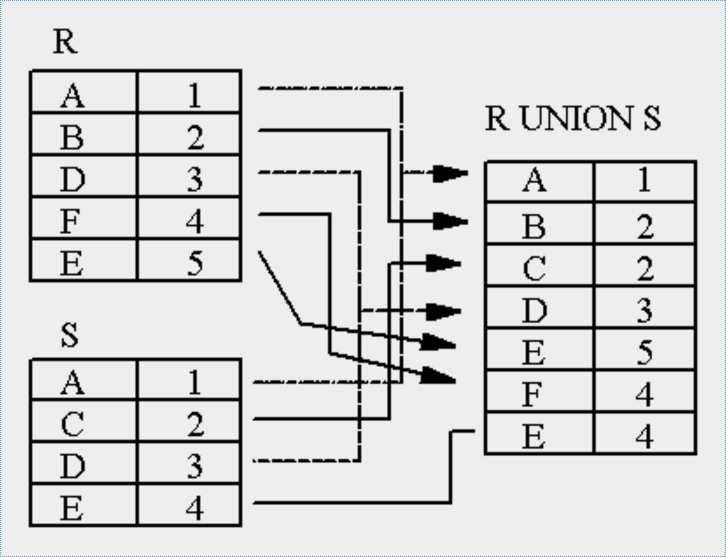
\includegraphics[width=.31\textwidth]{figs/spm6/unionexample}\hfill
	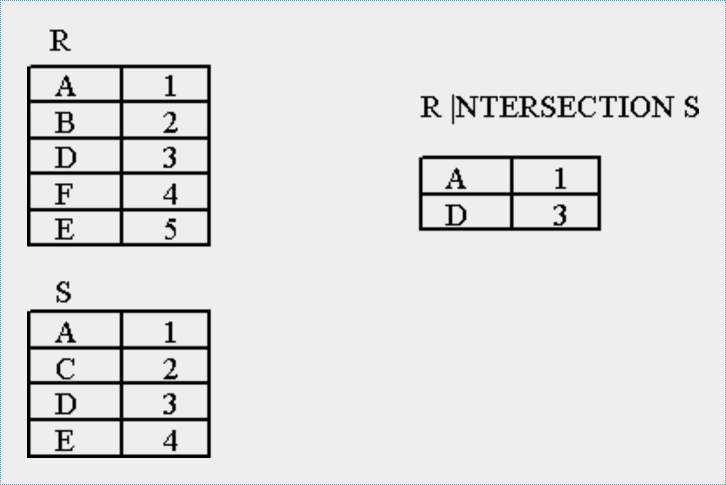
\includegraphics[width=.35\textwidth]{figs/spm6/intersectionexample}\hfill
	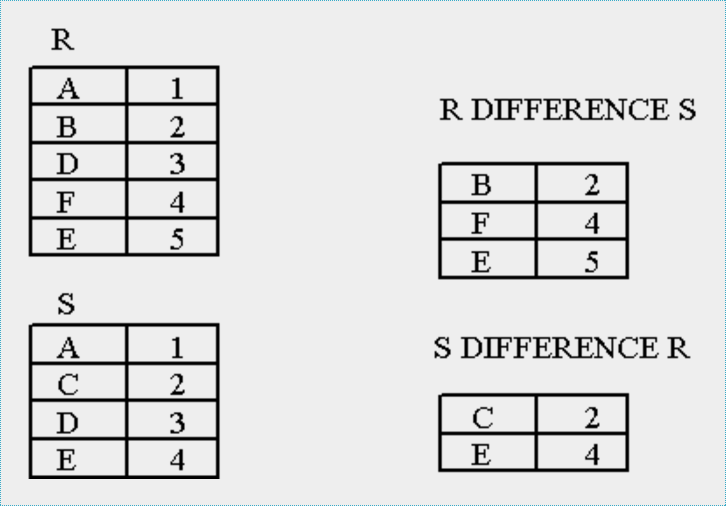
\includegraphics[width=.33\textwidth]{figs/spm6/differenceexample}	
	\caption{UNION (tv), INTERSECTION (midt) og DIFFERNENCE (tv).}
	\label{fig:union_intersection_difference_example}	
\end{figure}